\documentclass{beamer}
\usepackage[utf8]{inputenc}
\usepackage[spanish]{babel} %Permite definir el idioma del dcumento
%\usepackage[dvips]{epsfig}
%\usepackage[dvips]{graphicx}
\usepackage{url}
\usepackage{ulem}
\usepackage{beamerthemesplit}
\usepackage{moreverb}
\usepackage{color}
\usepackage{listings}
%\usetheme{Warsaw}
\usetheme{Frankfurt}

\title{Why Computer Architecture Matters}
\subtitle{``Memory Access''} 
\author[I. Villacura/R. Fernández/G. Zamora/C. Maureira/]{Ignacio Villacura\\Rodrigo Fernández\\Gabriel Zamora\\Cristián Maureira}
\date{\today}
%\institution[UTFSM]{Universidad Técnica Federico Santa María}

\begin{document}
\frame
{
	\titlepage
}

\frame
{
	\tableofcontents
}

\section{Introducción}
\frame
{
\frametitle{Documentos}
 \begin{itemize}
  \item Serie de 3 Papers.
  \item Cada uno abarca distintas técnicas de como mejorar el desempeño del código.
  \item Nuestra investigación se basa en el segundo documento.
\begin{itemize}
\item \textit{Pancratov C., Kurzer J.M., Shaw K.A., and Trawick M.L. Why computer architecture matters: Memory access. Computing in Science \& Engineering, 10, 2008.}
\end{itemize}
  \item Desde el primero obtenemos información base para entender el desarrollo de nuestra investigación.
 \end{itemize}
}

\frame
{
\frametitle{Why Computer Architecture Matters I}
\begin{itemize}
	\item Idea Principal:
	\begin{itemize}
		\item Mejorar el desempeño de los programas utilizando técnicas para utilizar de mejor manera la memoria Cache o técnicas para acelerar el calculo de funciones(Cos, Sen, Sqrt)
	\end{itemize}
	\item Ejemplo Base de la investigación
\end{itemize}
}
\frame
{
\frametitle{Un Ejemplo Concreto}
Muchos materiales consisten en pequeños cristales, cada uno de ellos orientados en una dirección
aleatoria.\\
La idea es calcular la diferencia promedio de todos los ángulos que se encuentran a una misma distancia entre dos
puntos (cristales) del material. Cada cristal esta definido por $(x,y,\theta)$, para los cuales definimos la funci\'on de correlaci\'on
 $g_{ij} = cos(6(\theta_i - \theta_j))$.
\begin{center}
	\includegraphics[scale=0.5]{img/cristales}
\end{center}
}

\frame[containsverbatim]
{
\frametitle{Código Base}
\begin{block}{}
\begin{verbatimtab}
for(i=0; i<N; ++i) //for each i < N
 for(j=i+1; j<N; ++j) {
  Dx = x[i]-x[j];
  Dy = y[i]-y[j];
  r = sqrt(Dx*Dx+Dy*Dy);
  g[r] += cos(6*(theta[i]-theta[j]));
  ++count[r]; 
 } 

for(r=0; r<MAX_r; ++r)
 g[r] = g[r]/count[r];
\end{verbatimtab}
\end{block}
}

\frame
{
\frametitle{Mejoras}

\begin{itemize}
\item  Para Mejorar el desempeño
\begin{itemize}

\item Se removió del loop principal, el cálculo de las funciones $cos$ y $sen$ ya que tienen unas latencias muy altas
\item El cálculo se realizará antes,  y se guardarán los resultados en arreglos, los cuales son accedidos con mayor rápidez que calcular el valor en el loop.
\item Esta técnica se le llama ``Precalcular Valores''

\end{itemize}
\end{itemize}
\begin{center}
\begin{tabular}{|l|l|l|}
\hline
& Normal & Optimización\\
\hline
Tiempo ejecución [s] & 143 & 55\\
\hline
\end{tabular}
\end{center}
}

\frame[containsverbatim]
{
  \frametitle{Código Base Mejorado}

\begin{block}{}
\begin{verbatimtab}
for(ii=0; ii<N; ++ii) {
 sin6[ii] = sin(6*theta[ii]);
 cos6[ii] = cos(6*theta[ii]);
}

for(i=0; i<N; ++i)
 for(j=i+1; j<N; ++j) {
  Dx = x[i]-x[j];
  Dy = y[i]-y[j];
  r = sqrt(Dx*Dx+Dy*Dy);
  g[r] += cos6[i]*cos6[j]+sin6[i]*sin6[j];
  ++count[r];
 }
\end{verbatimtab}
\end{block}
}

\section{Aspectos Importantes}
\frame
{
\frametitle{Memoria Principal}
\begin{itemize}
\item Existen 2 tipos:
\begin{itemize}
\item RAM o ``Random Access Memory'': Memoria que almacena datos de forma temporal. Es volátil, osea necesita energía continua.
\item ROM o ``Read Only Memory'': Viene escrita desde fabrica y se divide en 2 partes:
\begin{itemize}
\item POST o ``Power On Self Test'': Rutina de arranque
\item BIOS o ``Basic Input-Output System'': Permite activación de dispositivos de entrada o salida.
\end{itemize}
\end{itemize}
\item La CPU se conecta a esta memoria mediante un BUS de datos.
\end{itemize}
}
\frame
{
\frametitle{Memoria Caché}
\begin{itemize}
	\item<1->\textcolor{blue}{¿Qué es?}\\
		Sistema especial de almacenamiento de alta velocidad.
	\item<2->\textcolor{blue}{¿Cuál es su función principal?}\\
		Retener los datos utilizados recientemente.
	\item<3->\textcolor{blue}{¿Es efectivo?}\\
		Sí, dado que los programas acceden una y otra vez a los mismos datos o instrucciones.
	\item<4->\textcolor{blue}{¿Soluciona algún problema en especial?}\\
		Soluciona el problema de la alta latencia provocado por la lentitud de la memoria principal.
\end{itemize}
}
\frame
{
\frametitle{Memoria Caché}
\begin{columns}
	\begin{column}{0.4\textwidth}
		\includegraphics[width=5cm]{img/figura1.png}
	\end{column}
	\begin{column}{0.6\textwidth}
		\begin{itemize}
			\item<1->Leer desde el cache \emph{L1} es muy \textcolor{red}{rápido},pero leer desde la \emph{memoria principal} es más \textcolor{red}{lento}
			\item<2->Queremos \textcolor{red}{evitar} ir a la \emph{memoria principal} a toda costa
			\begin{itemize}
				\item<3->El cache L1 debe ser \textcolor{red}{capaz} de satisfacer tantos accesos a memoria como sea posible.
			\end{itemize}
			\item<4->\emph{Retener} datos en la memoria caché (datos estarán cuando la necesitemos).
		\end{itemize}
	\end{column}
\end{columns}
}

\frame
{
\frametitle{Localidad}
\begin{itemize}
	\item<1->\textcolor{red}{No} es posible retener los datos por un tiempo indefinido
	\item<2->\textcolor{blue}{Localidad Temporal}
	\begin{itemize}
		\item<3->Se busca \emph{reutilizar datos} todas las veces posibles en un tiempo corto.(datos más recientes)
	\end{itemize}
	\item<4->\textcolor{blue}{Localidad Espacial}
	\begin{itemize}
		\item<5->Corresponde a cuando un programa \textcolor{red}{usa} varias partes de datos que han sido guardados \emph{contiguos} en un periodo corto de tiempo.
	\end{itemize}
\end{itemize}
}
\frame
{
\frametitle{Localidad}
\begin{columns}
	\begin{column}{0.4\textwidth}
		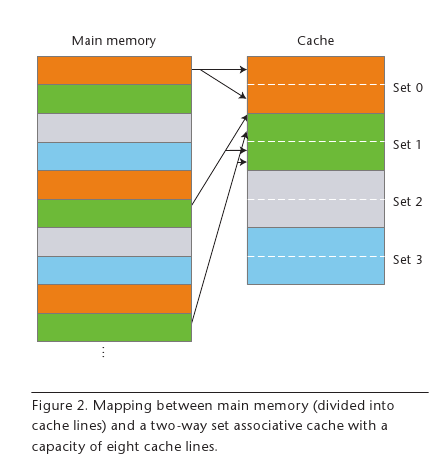
\includegraphics[width=5cm]{img/figura2.png}
	\end{column}
	\begin{column}{0.6\textwidth}
		\begin{itemize}
			\item<1->Las áreas en la memoria principal pueden mapear sólo dos líneas de cache.
			\item<2->Si mas de dos áreas mapean el mismo conjunto, resulta un \textcolor{red}{conflicto}, causando que algunos datos sean desalojados.
			\begin{itemize}
				\item<3->Podemos evitarlo con ayuda de la \emph{localidad espacial}
				\item<4->Áreas contiguas en la memoria principal garantizan un mapeo a \emph{diferentes} conjuntos en el cache.
			\end{itemize}
		\end{itemize}
	\end{column}
\end{columns}
}

\section{Objetivos Principales}
\frame
{
\frametitle{Motivación}
\begin{center}
	\Huge Una pequeña mejora, puede provocar grandes cambios
\end{center}
}

\subsection{Mejorando la localidad espacial}
\frame
{
\frametitle{``Array Merging''}
	Es una técnica que se utiliza para mejorar el tiempo de acceso a los datos en la
	memoria principal, haciendo mejor uso de la memoria caché
}
\frame[containsverbatim]
{
\frametitle{``Array Merging''}
	Inicialmente tenemos:
	\begin{block}{}
		\begin{verbatimtab}
		int x[N], y[N];
		float sin6[N], cos6[N];
		int count[MAX_R];
		float g[MAX_R];
		\end{verbatimtab}
	\end{block}
}

\frame
{
\frametitle{``Array Merging''}
	\begin{center}
		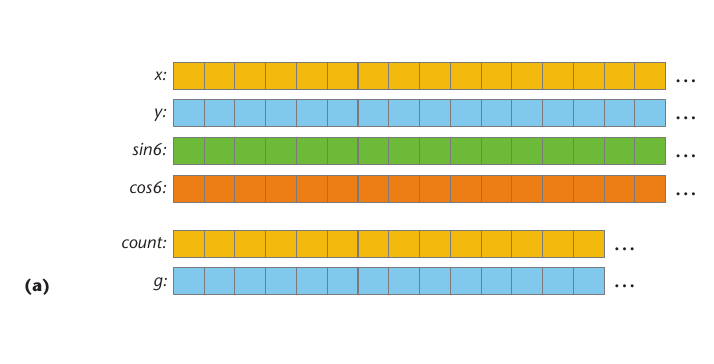
\includegraphics[scale=0.4]{../informe/images/array-1.png}
	\end{center}
	\begin{itemize}
		\item Datos son almacenados secuencialmente
		\item Ideal para procesar datos desde el arreglo x o y o el resto, pero no de todos
		\item Sin embargo, nuestro algoritmo hace uso de un dato de cada arreglo en cada iteración
	\end{itemize}		
}
\frame[containsverbatim]
{
\frametitle{``Array Merging''}
	Implementando localidad espacial:\\
	\begin{block}{}
		\begin{verbatimtab}
		struct DataStruct {
		int x, y;
		float cos6, sin6; };
		DataStruct data[N];
		\end{verbatimtab}
	\end{block}
	\begin{block}{}
		\begin{verbatimtab}
		struct AccumulationStruct {
		int count;
		float g; };
		AccumulationStruct accum[MAX_R];
		\end{verbatimtab}
	\end{block}
}

\frame
{
\frametitle{``Array Merging''}
	\begin{center}
		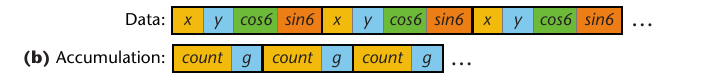
\includegraphics[scale=0.6]{../informe/images/array-2.png}
	\end{center}
	\begin{itemize}
		\item En la i-esima iteración, tenemos los datos necesarios, en forma secuencial
		\item Cuando el caché almacena el bloque de datos donde se encuentra x, almacena a los contiguos
		\item Dependiendo del tamaño de la linea de caché, podría incluso almacenar los datos para las iteraciones i+1 $\ldots$
	\end{itemize}		
}

\frame[containsverbatim]
{
\frametitle{``Array Merging''}
	Algoritmo implementado con Array Merging:
	\begin{block}{}
		\begin{verbatimtab}
for(i=0; i<N; ++i)
	for(j=i+1; j<N; ++j)
	{
		Dx = data[i].x - data[j].x;
		Dy = data[i].y - data[j].y;
		r = sqrt(Dx*Dx + Dy*Dy);
		accum[r].g += data[i].cos6 * data[j].cos6
		+ data[i].sin6 * data[j].sin6;
		++accum[r].count;
	}
		\end{verbatimtab}
	\end{block}
}

\frame
{
\frametitle{Resultados}
\begin{center}
\begin{tabular}{|l|l|l|}
\hline
& Normal & Optimización\\
\hline
Tiempo ejecución [s] & 143 & 54\\
\hline
\end{tabular}
\end{center}

}


\subsection{Mejorando la localidad temporal}
\frame
{
\frametitle{``Blocking''}
	\begin{center}
		\includegraphics[scale=0.4]{img/blocking}
	\end{center}
	Queremos agrupar las variables de tal forma que quepan fácilmente en el caché de menor nivel.\\
	Buscamos realizar más computaciones por cada dato que extraemos de la memoria principal.

%Para eso, ordenamos el código en bloques 
}

\frame[containsverbatim]
{
\frametitle{Blocking: Como lo hacemos?}

	Depende del programa y algoritmo que vallamos a optimizar.\\
	Recordemos como se estructuraba la ejecución de nuestro código:
\tiny
	\begin{block}{}
		\begin{verbatimtab}
for(i=0; i<N; ++i)
	for(j=i+1; j<N; ++j)
	{
		Dx = x[i]-x[j];
		Dy = y[i]-y[j];
		r = sqrt(Dx*Dx+Dy*Dy);
		g[r] += cos(6*(theta[i]-theta[j]));
		++count[r]; 
	} 

for(r=0; r<MAX_r; ++r)
	g[r] = g[r]/count[r];
		\end{verbatimtab}
	\end{block}
\normalsize
}


\frame[containsverbatim]
{

	Entonces, cambiamos las iteraciones para que corran por bloques:
\tiny
	\begin{block}{}
		\begin{verbatimtab}
for(A = 0; A+2*blocksize < N; A+= blocksize)
{
	for(B=A+blocksize; B+blocksize<N; B+=blocksize)
	{
		for(i=A; i<A+blocksize; ++i)
		{
			for(j=B; j<B+blocksize; ++j)
			{
				(...)
			}
		}
	}
}
(...)
		\end{verbatimtab}
	\end{block}
\normalsize
Esto claramente al la vez trae otras consecuencias...
}

\frame
{
\frametitle{Desventajas del ``Blocking''}
\begin{itemize}
	\item<1-> Aumenta la complejidad del código.
	\item<2-> Hace falta la implementación de más código para el manejo de los casos especiales. 
	\begin{itemize}
		\item<3-> Rangos fuera de los índices.
		\item<4-> Evitar que falten o se repitan operaciones.
	\end{itemize}
\end{itemize}
	\begin{center}
		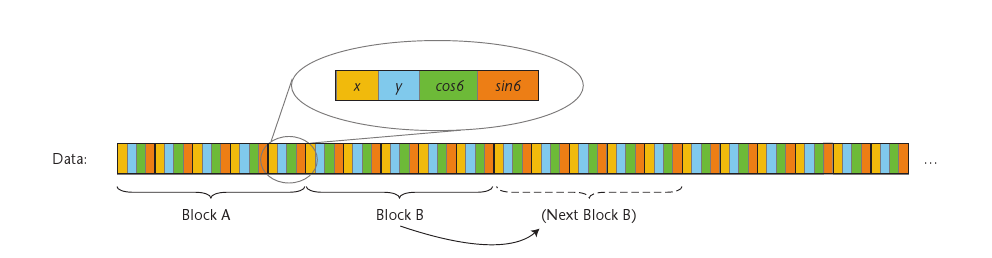
\includegraphics[scale=0.4]{img/figure4}
	\end{center}
}

\frame
{
El ejemplo que teníamos no incluía los ``casos especiales''...\\

Probamos varias formas, hasta que logramos hacer una que si realizaba todas las operaciones, pero...
}
\frame[containsverbatim]
{
\frametitle{Nuestra implementación de ``Blocking''}
\tiny
\begin{block}{}
		\begin{verbatimtab}
	for(A=0; A<N; A+=blocksize)
	{
		C=A;
		for(B=A,flag=1; B<N; B+=blocksize,flag=0)
		{
			for(i=A; i<A+blocksize; ++i)
			{	
				if(flag)
				{
					C++;
					for(j=C; j<B+blocksize; ++j)
					{
						(...)
					}
				}
				else
					for(j=B; j<B+blocksize; ++j)
					{
						(...)
					}
			}
			C=B;
		}
	}
(...)
		\end{verbatimtab}
\end{block}
\normalsize
}

\frame
{
\frametitle{Resultados de nuestro ``Blocking''}

En algunos casos de prueba se mantuvo el tiempo de procesamiento.
En otros, aumentó el tiempo de procesamiento en comparación con el código original.
En promedio, no se detectaron mejoras sustanciales en comparación con el método anterior.
Posibles causas de este resultado:
\begin{itemize}
	\item Nuestro hardware ya estaba haciendo un excelente trabajo.
	\item El aumento de operaciones por cada ciclo no se compensaba.
\end{itemize}
}
\frame
{
\frametitle{Resultados}
\begin{center}
\begin{tabular}{|l|l|l|}
\hline
& Normal & Optimización\\
\hline
Tiempo ejecución [s] & 143 & 54\\
\hline
\end{tabular}
\end{center}
}


\subsection{Mejoras propuestas}
\frame
{
\frametitle{Mejoras propuesta en nuestra investigación}
	\begin{itemize}
		\item Aproximación de raíces
		\item Aproximación de funciones trigonométricas
	\end{itemize}
}
\frame
{
\frametitle{Aproximación de raíces}
	\begin{itemize}
		\item<1->Utilizando una \textcolor{blue}{Lookup table}
		\begin{itemize}
			\item<1->Es una estructura de datos, usualmente un arreglo.
			\item<1->Usada para reemplazar un cálculo en tiempo de ejecución con una simple operación de indexación en un arreglo.
		\end{itemize}
		\item<1->Recordando el ejemplo de \textcolor{red}{Array Merging}
	\end{itemize}
}

\begin{frame}[fragile]
		\normalsize
		\textcolor{blue}{Original}
		\tiny
		\begin{lstlisting}[language=C]
			for(j=i+1; j<N; ++j)
			{
			Dx = data[i].x - data[j].x;
			Dy = data[i].y - data[j].y;
		\end{lstlisting}
		\vspace{-0.1cm}
			\textcolor{red}{r = sqrt(Dx*Dx + Dy*Dy);}
		\vspace{-0.1cm}
		\begin{lstlisting}[language=C]
			accum[r].g += data[i].cos6 * data[j].cos6 + data[i].sin6 * data[j].sin6;
			++accum[r].count;
			}
		\end{lstlisting}
		\normalsize
		\textcolor{blue}{Modificado}
		\tiny
		\begin{lstlisting}[language=C]
			for(j=i+1; j<N; ++j)
			{
			Dx = data[i].x - data[j].x;
			Dy = data[i].y - data[j].y;
		\end{lstlisting}
		\vspace{-0.1cm}
			\textcolor{red}{root(Dx*Dx + Dy*Dy, r)}
		\vspace{-0.1cm}
		\begin{lstlisting}[language=C]
			accum[r].g += data[i].cos6 * data[j].cos6 + data[i].sin6 * data[j].sin6;
			++accum[r].count;
			}
		\end{lstlisting}
\end{frame}

\begin{frame}[fragile]
	\normalsize
	Miremos ahora \textcolor{blue}{tabla.h}, donde está la definición de \textcolor{red}{root()}.
	\scriptsize
	\begin{lstlisting}[language=C]
	#define root(x,y) \
	switch(x) { \
		case 0: y = 0; break; \
		case 1: y = 1; break; \
		case 2: y = 1; break; \
		case 3: y = 1; break; \
		(...)
		case 997: y = 31; break; \
		case 998: y = 31; break; \
		case 999: y = 31; break; \
	}
	\end{lstlisting}
\end{frame}

\frame
{
\frametitle{Aproximación de funciones trigonométricas}
	\small
	\begin{itemize}
		\item<1->Buscamos poder \textcolor{blue}{optimizar} el cálculo de las funciones trigonométricas.
		\item<2->Recordemos nuestras queridas \textcolor{blue}{Series de Taylor}.
		\item<3->$\operatorname{sin}{x}= \sum^{\infty}_{n=0} \frac{(-1)^n}{(2n+1)!} x^{2n+1} = x - \frac{x^3}{3!} + \frac{x^5}{5!} - \cdots $
		\item<4->Algunos computadores, no pueden calcular el \textcolor{blue}{seno} de un valor dado.
		\item<5->En vez de eso, ocupan una fórmula basada en las \textcolor{blue}{Series de Taylor} para calcular el valor con una gran precisión (para valores de x cercanos a 0)
		\item<6->$\operatorname{sin}(x) \approx x - \frac{x^3}{6} + \frac{x^5}{120} - \frac{x^7}{5040}$
	\end{itemize}
}

\frame
{
\frametitle{Aproximación de funciones trigonométricas}
	\small
	\begin{itemize}
		\item<1->Pero, ocupamos \textcolor{red}{muchas} multiplicaciones para calcular los $x^k$
		\item<2->Utilizaremos la esencia del \textcolor{blue}{Algoritmo de Horner}
		\begin{itemize}
			\item<3-> Algoritmo para evaluar de forma eficiente polinomios de una forma monomial.
			\item<3-> \scriptsize $ p(x) = a_0 + a_1 x + a_2 x^2 + a_3 x^3 + \cdots + a_n x^n $
		\end{itemize}
		\item<4->Por lo tanto podremos reducir nuestro polinomio:
			$$\operatorname{sin}(x) \approx x - \frac{x^3}{6} + \frac{x^5}{120} - \frac{x^7}{5040}$$
			a,
			$$\operatorname{sin}(x) \approx x \left( 1 - x^{2}\left(\frac{1}{6} + x^{2}\left(\frac{1}{120} - \frac{x^2}{5040}\right)\right)\right)$$
		\item<5->Reduciendo el numero de multiplicaciones de \textcolor{blue}{12} a \textcolor{blue}{3}
		\item<6->Lamentablemente el efectuar ésta operación, se transforma en un cálculo muy caro, especialmente para procesadores lentos.
	\end{itemize}
	
}

\section{Thinking through trade-offs in your code}
\frame
{
\frametitle{Continuación de nuestro trabajo}

\begin{itemize}
	\item Ahonda más en el problema.
	\item Busca optimizaciones especialmente diseñadas para ese algoritmo.
	\item<1-> Lo que interesa es encontrar el ``cuello de botella'' que limita la velocidad.
	\begin{itemize}
		\item<2-> Diferentes estrategias para eliminar la raíz cuadrada.
		\item<3-> Mejorar la localidad espacial ordenando los datos antes de procesarlos.
		\item<4-> Mejorar el código de tal forma de aprovechar como el procesador maneja las
operaciones aritméticas.
	\end{itemize}
\end{itemize}


}


\frame
{
\begin{center}
\begin{Huge}\textit{¿Preguntas?}\end{Huge}
\end{center}
}

\end{document}
